\chapter{The NetDiag Web Application}

\section{Application Purpose and Design}

NetDiag is a containerized network diagnostic web tool that exposes \texttt{ping} functionality over HTTP via a minimal Flask application. It exists in this lab not as a contrived toy, but as a faithful model of a class of vulnerable applications that appear regularly in real infrastructure: network appliance web interfaces, internal DevOps tooling, and monitoring dashboards built quickly without security review.

The application mirrors patterns found in router and managed switch web UIs that expose diagnostic commands such as \texttt{ping}, \texttt{traceroute}, and \texttt{nslookup} to authenticated or unauthenticated users. It also reflects the internal tooling pattern: a developer needs a quick way to test connectivity from a server, writes a Flask wrapper around a shell command, and deploys it on the internal network without ever intending it to be a security boundary.

The entire application lives in a single file, \texttt{app.py}, with one vulnerable route. Every design decision in the application is intentional for demonstration purposes, but each one mirrors a real misconfiguration:

\begin{itemize}
    \item Arbitrary user input is accepted via a query parameter with no validation.
    \item Input is passed directly to the shell via \texttt{os.popen()}.
    \item The process runs as \texttt{root} inside the container — no \texttt{USER} directive appears in the Dockerfile.
    \item Raw command output is returned to the browser.
    \item No authentication, input validation, or rate limiting is implemented.
\end{itemize}

The vulnerability class is \textbf{OS Command Injection} (CWE-78): user-supplied input is embedded in a shell command string and interpreted by \texttt{/bin/sh}. The attack surface is a single HTTP GET endpoint, unauthenticated, exposed on port 5000.

\section{Flask and the WSGI Model}

\subsection{WSGI: The Bridge Between Network and Python}

Flask is a WSGI application. WSGI --- the Web Server Gateway Interface, defined in PEP 3333 --- is the Python standard that defines how a web server hands an HTTP request to a Python application. Any WSGI-compliant application implements a callable with the signature \texttt{\_\_call\_\_(environ, start\_response)}. The web server calls this callable for each request; the application returns an iterable of response bytes.

In development, Flask uses Werkzeug's built-in WSGI server, started via \texttt{flask run} or \texttt{app.run()}. In production, a WSGI application would sit behind gunicorn or uWSGI. NetDiag uses the development server, which is single-threaded by default.

\subsection{Flask Request Lifecycle}

Each HTTP request to NetDiag follows this path:

\begin{enumerate}
    \item A TCP connection is accepted on port 5000.
    \item Werkzeug parses the HTTP request and populates the \texttt{request} context object.
    \item The URL router matches the path to the registered view function via \texttt{@app.route}.
    \item The view function executes and returns a response string or object.
    \item Werkzeug serializes the HTTP response, sends it over the socket, and closes the connection.
\end{enumerate}

\subsection{OS-Level View of Request Handling}

At the operating system level, the Flask development server runs as a single Python process. When the \texttt{/ping} route calls \texttt{os.popen()}, the following kernel operations occur:

\begin{enumerate}
    \item The Flask process (UID 0) calls \texttt{pipe()}, creating a read/write file descriptor pair.
    \item The Flask process calls \texttt{fork()}, creating a child process that inherits UID 0.
    \item The child calls \texttt{dup2()} to redirect its stdout to the write end of the pipe.
    \item The child calls \texttt{execve("/bin/sh", ["-c", cmd], environ)}.
    \item The shell executes the command string.
    \item The parent reads the pipe via \texttt{os.popen().read()}, blocking until the child exits.
\end{enumerate}

The resulting process tree during a request looks like this:

\begin{lstlisting}
python3 app.py (PID X, UID 0)
  /bin/sh -c "ping -c 3 <user_input>" (PID X+1, UID 0)
      ping / injected command (PID X+2, UID 0)
\end{lstlisting}

Because the container runs without user namespace remapping, UID 0 inside the container is UID 0 on the host kernel. Every forked process inherits this identity. Injected commands therefore execute with full root privileges.

\begin{lstlisting}
# Verify Flask process UID inside container
ps aux

# Verify port binding
ss -tlnp | grep 5000
\end{lstlisting}

\begin{figure}[h]
\centering
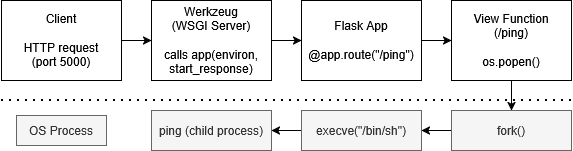
\includegraphics[width=\textwidth]{images/ch5/wsgi_execution_flow.png}
\caption{Flask Request to OS Process: WSGI Execution Flow. Shows HTTP request arriving at Werkzeug, dispatched to Flask route, \texttt{os.popen()} called, \texttt{fork()} and \texttt{execve("/bin/sh")} fired, child process spawned. UID 0 inheritance annotated at the fork boundary.}
\end{figure}

\section{Route Structure and Request Handling}

NetDiag exposes two routes:

\begin{itemize}
    \item \texttt{GET /} --- serves the HTML UI form page; no user input is processed.
    \item \texttt{GET /ping?host=<value>} --- the vulnerable route; processes the \texttt{host} query parameter.
\end{itemize}

The attack surface is intentionally narrow: one route, one parameter. But that single route is the critical path.

\subsection{Input Handling in \texttt{/ping}}

Flask extracts the \texttt{host} value using \texttt{request.args.get('host')}. Werkzeug parses query parameters into an \texttt{ImmutableMultiDict} object. URL-encoded characters are decoded automatically before the value reaches the view function:

\begin{itemize}
    \item \texttt{\%3B} decodes to \texttt{;}
    \item \texttt{\%26} decodes to \texttt{\&}
    \item \texttt{\%7C} decodes to \texttt{|}
\end{itemize}

This decoding happens transparently. The attacker sends URL-encoded shell metacharacters in the query string; the application receives the decoded, shell-active characters. There is no type checking, no length limit, and no character filtering at any point in this pipeline.

The HTTP method is GET: input travels in the URL, appears in server access logs, and is stored in browser history. No CSRF protection is relevant for a read-only GET --- though the "read-only" assumption breaks entirely once command injection is achieved.

Both successful and failed requests return \texttt{200 OK}. Error output is not surfaced, but stdout from all commands in the injection chain is included in the response body.

\begin{lstlisting}
# Normal request
curl "http://192.168.98.4:5000/ping?host=8.8.8.8"

# Semicolon injected via URL encoding
# %3B decodes to ; before reaching app.py
curl "http://192.168.98.4:5000/ping?host=8.8.8.8%3Bid"
\end{lstlisting}

\section{The Vulnerable \texttt{/ping} Route: Code Walkthrough}

\subsection{The Vulnerable Code}

\begin{lstlisting}[language=Python]
@app.route('/ping')
def ping():
    host = request.args.get('host', '')
    result = os.popen("ping -c 3 " + host).read()
    return render_template('index.html', result=result)
\end{lstlisting}

Three lines. Each one contributes to the vulnerability.

\subsection{Line-by-Line Analysis}

\textbf{\texttt{host = request.args.get('host', '')}}

Retrieves the raw decoded string value of the \texttt{host} query parameter. If the parameter is absent, defaults to an empty string. No validation, sanitization, or type enforcement is applied. The value at this point may contain any character, including shell metacharacters.

\textbf{\texttt{os.popen("ping -c 3 " + host)}}

This is the vulnerability. String concatenation builds a shell command. The result is passed as a single string to \texttt{/bin/sh -c}. The shell receives and interprets the entire string, including any metacharacters embedded in \texttt{host}. \texttt{os.popen()} returns a file-like object connected to the command's stdout via a pipe.

\textbf{\texttt{.read()}}

Reads the entire stdout of the shell session into a Python string. This is a blocking call: the Flask thread waits until all processes in the shell's command chain have exited. Critically, it captures output from \emph{all} commands that execute --- including injected ones.

\textbf{\texttt{render\_template('index.html', result=result)}}

Injects the captured output into the HTML template and returns it in the HTTP response. The attacker sees the results of injected commands directly in the browser.

\subsection{Shell Metacharacter Interpretation}

When \texttt{/bin/sh} receives the concatenated command string, it interprets the following metacharacters:

\begin{itemize}
    \item \texttt{;} --- command separator: both commands run sequentially regardless of exit status.
    \item \texttt{\&\&} --- conditional AND: second command runs only if the first succeeds.
    \item \texttt{||} --- conditional OR: second command runs only if the first fails.
    \item \texttt{|} --- pipe: stdout of first command becomes stdin of second.
    \item \texttt{`...`} or \texttt{\$()} --- command substitution.
    \item \texttt{\&} --- background execution.
    \item \texttt{\textbackslash n} --- newline also acts as a command separator.
\end{itemize}

\subsection{Kernel-Level Execution for \texttt{8.8.8.8;id}}

Tracing the full kernel execution path for the input \texttt{8.8.8.8;id}:

\begin{enumerate}
    \item \texttt{os.popen("ping -c 3 8.8.8.8;id")} is called in the Flask process (PID X, UID 0).
    \item Python calls \texttt{pipe()} to create a read/write file descriptor pair.
    \item Python calls \texttt{fork()}: child process PID X+1 is created, inheriting UID 0.
    \item Child calls \texttt{dup2()} to redirect its stdout to the write end of the pipe.
    \item Child calls \texttt{execve("/bin/sh", ["-c", "ping -c 3 8.8.8.8;id"], environ)}.
    \item The shell parses the command string, identifies the \texttt{;} separator, and runs \texttt{ping}, then \texttt{id}.
    \item \texttt{id} produces \texttt{uid=0(root) gid=0(root) groups=0(root)} on stdout, which is written to the pipe.
    \item The parent process reads the pipe via \texttt{.read()}, receives the combined output, and the Flask response includes the \texttt{id} output.
\end{enumerate}

The root cause is unambiguous: \textbf{unsanitized user input is used as the content of a shell command string argument}.

\begin{lstlisting}
# Confirm command injection with id
curl "http://192.168.98.4:5000/ping?host=8.8.8.8%3Bid"
# Response contains: uid=0(root) gid=0(root)

# Enumerate environment variables
curl "http://192.168.98.4:5000/ping?host=8.8.8.8%3Benv"

# Read /etc/passwd
curl "http://192.168.98.4:5000/ping?host=8.8.8.8%3Bcat+/etc/passwd"

# Confirm docker.sock presence
curl "http://192.168.98.4:5000/ping?host=8.8.8.8%3Bls+-la+/var/run/docker.sock"
\end{lstlisting}

\section{Why \texttt{os.popen()} is Dangerous}

\subsection{\texttt{os.popen()} Internals}

\texttt{os.popen(cmd)} is a thin Python wrapper around the C library \texttt{popen()} function. Internally it invokes \texttt{/bin/sh -c <cmd\_string>}, treating the entire argument as a shell script. The syscall chain is:

\begin{lstlisting}
pipe() -> fork() -> execve("/bin/sh", ["-c", cmd_string], environ)
\end{lstlisting}

The shell receives full interpretation authority over \texttt{cmd\_string}. Any metacharacters present --- regardless of whether they were intended by the developer --- are active. When user input is embedded in \texttt{cmd\_string} via string concatenation, the user effectively controls the content of a shell script.

\texttt{os.popen()} is deprecated in Python 3. The \texttt{subprocess} module is the documented replacement, but the choice between safe and unsafe use of \texttt{subprocess} requires understanding the distinction between string and list invocation.

\subsection{Safe Alternative: \texttt{subprocess.run()} with List Argument}

\begin{lstlisting}[language=Python]
import subprocess
result = subprocess.run(
    ['ping', '-c', '3', host],
    capture_output=True, text=True, timeout=10
)
\end{lstlisting}

When \texttt{subprocess.run()} receives a list, each element is treated as a discrete argument. No shell is invoked. The syscall chain becomes:

\begin{lstlisting}
fork() -> execve("/bin/ping", ["ping", "-c", "3", host], environ)
\end{lstlisting}

\texttt{/bin/ping} is called directly. There is no shell to interpret metacharacters. If \texttt{host} contains \texttt{8.8.8.8;id}, the string \texttt{8.8.8.8;id} is passed as a literal argument to \texttt{ping}, which rejects it as an invalid hostname. The injected command never executes.

\subsection{The \texttt{shell=True} Trap}

\begin{lstlisting}[language=Python]
# Still vulnerable -- identical to os.popen()
subprocess.run("ping -c 3 " + host, shell=True)
\end{lstlisting}

Passing \texttt{shell=True} to \texttt{subprocess.run()} re-introduces \texttt{/bin/sh -c} and restores the identical vulnerability. This is a common mistake: a developer switches from \texttt{os.popen()} to \texttt{subprocess} in response to a security finding, but retains \texttt{shell=True}, achieving nothing.

\subsection{Comparison}

\begin{center}
\begin{tabular}{|l|c|c|c|}
\hline
\textbf{Method} & \textbf{Shell Invoked} & \textbf{Metachar Interpreted} & \textbf{Vulnerable} \\
\hline
\texttt{os.popen(string)} & Yes (\texttt{/bin/sh -c}) & Yes & Yes \\
\texttt{subprocess.run(string, shell=True)} & Yes (\texttt{/bin/sh -c}) & Yes & Yes \\
\texttt{subprocess.run(list)} & No (direct execve) & No & No \\
\texttt{subprocess.run(list, shell=False)} & No & No & No \\
\hline
\end{tabular}
\end{center}

\subsection{Input Validation as Defense-in-Depth}

Input validation is not a substitute for safe API usage, but it is a recommended additional layer. An allowlist approach restricts \texttt{host} to characters valid in IP addresses and hostnames:

\begin{lstlisting}[language=Python]
import re
if not re.match(r'^[a-zA-Z0-9.\-]+$', host):
    return "Invalid host", 400
\end{lstlisting}

This rejects any input containing \texttt{;}, \texttt{\&}, \texttt{|}, backticks, \texttt{\$}, parentheses, or newlines. Even if a future developer inadvertently reintroduces a shell invocation, the validation layer limits the blast radius.

\subsection{Output Reflection Amplifies Impact}

Because \texttt{os.popen().read()} captures the full stdout of the shell session and \texttt{render\_template} includes it in the HTTP response body, this is a \textbf{non-blind injection}. The attacker reads the output of injected commands directly in the browser. No out-of-band channel, timing oracle, or side-channel technique is required for enumeration. Only stderr is not captured by default; adding \texttt{2>\&1} to any injected command resolves this.

\begin{lstlisting}[language=Python]
# Demonstrate safe vs unsafe in Python REPL inside container
python3 -c "
import os, subprocess

# Unsafe: semicolon is interpreted
print(os.popen('echo safe; id').read())

# Safe: semicolon passed as literal argument
r = subprocess.run(['echo', 'safe; id'], capture_output=True, text=True)
print(r.stdout)  # prints: safe; id -- no command executed
"
\end{lstlisting}

\section{The HTML Template: UI Breakdown}

NetDiag's front end is a single Jinja2 template, \texttt{index.html}, served by \texttt{render\_template}. The form submits via \texttt{GET} to \texttt{/ping}, placing the \texttt{host} value in the query string.

Command output is rendered in the template using Jinja2's standard variable substitution: \texttt{\{\{ result \}\}}. Jinja2 auto-escapes HTML special characters in \texttt{.html} templates by default, which prevents the command output from being interpreted as HTML or executing JavaScript. This mitigates cross-site scripting in the output --- but it does not prevent command injection. The HTML escaping occurs \emph{after} the shell has already executed. The damage is done before the template is rendered.

If a \texttt{<pre>} tag wraps the output block, whitespace and newlines in command output are preserved, making multi-line results such as \texttt{/etc/passwd} or \texttt{env} readable in the browser without further formatting.

The absence of authentication on the route means the form is accessible to any client with network reach to port 5000. The absence of a CSRF token is technically irrelevant for a GET request but is a clear signal that no security review was applied to this application.

The practical consequence of output reflection is significant: this vulnerability requires no blind exploitation technique. The attacker submits a request, reads the response, and proceeds with full situational awareness.

\section{Running as Root Inside the Container}

\subsection{The Missing \texttt{USER} Directive}

The NetDiag Dockerfile does not specify a \texttt{USER} directive:

\begin{lstlisting}
FROM python:3.11-slim
WORKDIR /app
COPY . .
RUN pip install flask
CMD ["python3", "app.py"]
# No: USER nobody
\end{lstlisting}

When no \texttt{USER} directive is present, Docker defaults to running the container's main process as UID 0. This UID is inherited by every child process: Flask inherits it, \texttt{os.popen()} inherits it, the shell inherits it, and every injected command inherits it.

\subsection{UID 0 Without User Namespace Remapping}

Docker does not enable user namespace remapping by default. Without this feature, UID 0 inside the container maps directly to UID 0 on the host kernel. This can be confirmed from inside the container:

\begin{lstlisting}
# Confirm root inside container
docker exec netdiag-app id
# uid=0(root) gid=0(root) groups=0(root)

# Confirm direct UID mapping -- no user namespace in effect
docker exec netdiag-app cat /proc/self/uid_map
# 0          0 4294967295

# Verify socket permissions relative to container UID
docker exec netdiag-app ls -la /var/run/docker.sock
# srw-rw---- 1 root 132 ... -- UID 0 passes owner check
\end{lstlisting}

The output \texttt{0 0 4294967295} from \texttt{uid\_map} indicates that UID 0 inside the container maps to UID 0 on the host, covering the full UID range. There is no remapping layer.

\subsection{Impact on the Attack Chain}

Running as UID 0 is the second critical factor in the complete exploitation path (alongside the mounted \texttt{docker.sock}, discussed in Chapter~8):

\begin{itemize}
    \item Injected commands via the \texttt{/ping} route execute as root.
    \item \texttt{/var/run/docker.sock} has permissions \texttt{srw-rw----}, owned by \texttt{root:docker}. UID 0 passes the owner permission check and can read and write the socket directly.
    \item Installing additional tooling with \texttt{apt-get install docker.io} requires root --- this succeeds inside the container.
    \item Files written to the host filesystem via a container escape are owned by root on the host.
    \item The reverse shell spawned via the injected command (see Chapter~8) inherits UID 0, arriving with root privileges.
\end{itemize}

\subsection{What Running as Non-Root Would Change}

A non-root UID cannot read or write \texttt{/var/run/docker.sock} unless that UID is a member of the \texttt{docker} group --- which grants equivalent access and should be treated as root-equivalent. Without socket access, the container escape path documented in Chapter~8 is blocked. \texttt{apt-get install} would fail, preventing installation of the Docker CLI. Remote code execution via command injection would still be possible, but the ability to pivot to a full container escape would be substantially constrained.

\subsection{Correct Dockerfile Fix}

\begin{lstlisting}
RUN useradd -m -u 1001 appuser
USER appuser
# /var/run/docker.sock becomes inaccessible to UID 1001
\end{lstlisting}

This change, combined with the \texttt{subprocess} fix and input validation discussed in Section~5.5, is addressed in detail in Chapter~11.